% CVPR 2026 Paper Template; see https://github.com/cvpr-org/author-kit

\documentclass[10pt,twocolumn,letterpaper]{article}

%%%%%%%%% PAPER TYPE  - PLEASE UPDATE FOR FINAL VERSION
\usepackage{cvpr}              % To produce the CAMERA-READY version
% \usepackage[review]{cvpr}      % To produce the REVIEW version
% \usepackage[pagenumbers]{cvpr} % To force page numbers, e.g. for an arXiv version

% Import additional packages in the preamble file, before hyperref
%% This file contains a number of tweaks that are typically applied to the main document.
%% They are not enabled by default, but can be enabled by uncommenting the relevant lines.

%%
%% Inline annotations; for predefined colors, refer to "dvipsnames" in the xcolor package:
%% https://tinyurl.com/overleaf-colors
%%
\newcommand{\red}[1]{{\color{red}#1}}
\newcommand{\todo}[1]{{\color{red}#1}}
\newcommand{\TODO}[1]{\textbf{\color{red}[TODO: #1]}}
%%
%% disable for camera ready / submission by uncommenting these lines  
%%
% \renewcommand{\TODO}[1]{}
% \renewcommand{\todo}[1]{#1}

%%
%% work harder in optimizing text layout. Typically shrinks text by 1/6 of page, enable
%% it at the very end of the writing process, when you are just above the page limit
%%
% \usepackage{microtype}

%%
%% fine-tune paragraph spacing
%%
% \renewcommand{\paragraph}[1]{\vspace{.5em}\noindent\textbf{#1.}}

%%
%% globally adjusts space between figure and caption
%%
% \setlength{\abovecaptionskip}{.5em}


%%
%% Allows "the use of \paper to refer to the project name"
%% with automatic management of space at the end of the word
%%
% \usepackage{xspace}
% \newcommand{\paper}{ProjectName\xspace}

%%
%% Commonly used math definitions
%%
% \DeclareMathOperator*{\argmin}{arg\,min}
% \DeclareMathOperator*{\argmax}{arg\,max}

%%
%% Tigthen underline
%%
% \usepackage{soul}
% \setuldepth{foobar}
% Tighter space around floats, to fit the 2-page limit
\setlength{\textfloatsep}{8pt plus 2pt minus 2pt}
\setlength{\dbltextfloatsep}{8pt plus 2pt minus 2pt}
\setlength{\abovecaptionskip}{4pt}


% It is strongly recommended to use hyperref, especially for the review version.
% hyperref with option pagebackref eases the reviewers' job.
% Please disable hyperref *only* if you encounter grave issues, 
% e.g. with the file validation for the camera-ready version.
%
% If you comment hyperref and then uncomment it, you should delete *.aux before re-running LaTeX.
% (Or just hit 'q' on the first LaTeX run, let it finish, and you should be clear).
\definecolor{cvprblue}{rgb}{0.21,0.49,0.74}
\usepackage[breaklinks,colorlinks,allcolors=cvprblue]{hyperref}

%%%%%%%%% PAPER ID  - PLEASE UPDATE
\def\paperID{*****} % *** Enter the Paper ID here
\def\confName{CVPR}
\def\confYear{2026}

%%%%%%%%% TITLE - PLEASE UPDATE
\title{Region-Text Contrastive Grounding for Language-driven Grasp Detection}

%%%%%%%%% AUTHORS - PLEASE UPDATE
\author{Duc Anh Hoang\\
{\small Code: \url{https://github.com/hoangducanh1865/fpt_entrance_test}}
}

\begin{document}
\maketitle
\begin{abstract}
Most failures of a GR-ConvNet + CLIP baseline for language-driven grasp detection on Grasp-Anything++ grasp the wrong object.
We add a training-only region-text contrastive loss: features pooled over the prompted object's mask must match the prompt better than the other objects of the scene.
On the official split, it improves the baseline by 2.5 H points over three seeds, with a gain in every seed.
We also re-run LGD and the official baseline with the authors' code, and bound the grounding error with gates.
\end{abstract}

\section{Introduction}
\label{sec:intro}

Grasp-Anything++~\cite{vuong2024language} defines language-driven grasp detection: given an RGB image and a prompt such as ``pick up the pear by its stem'', predict a 2D grasp rectangle $g = (x, y, w, h, \theta)$ for a two-finger gripper.

Two vision-language models judged 1,000 failures of a reproduced GR-ConvNet + CLIP~\cite{kumra2020antipodal,vuong2024language} on an earlier split: 47\% grasp another object than the prompted one, 34\% have a wrong grasp on the right object.
Its loss says where to grasp, but nothing tells its encoder, trained from scratch, which object the prompt names.

We contribute (1) a training-only region-text contrastive loss with the other objects of the scene as negatives, (2) a three-seed evaluation on the official split, with LGD and the official baseline re-run, and (3) gates that measure how much grounding limits success.

\section{Related work}
\label{sec:related}

Grasp-Anything~\cite{vuong2023grasp} and Grasp-Anything++~\cite{vuong2024language} are large synthetic grasp datasets with part masks and prompts.
LGD~\cite{vuong2024language} and LLGD~\cite{nguyen2024lightweight} generate grasps with diffusion and consistency models; GraspMamba~\cite{nguyen2024graspmamba} fuses text and image at several levels with state-space models.
Closest to us, MaskGrasp~\cite{vo2024maskgrasp} feeds segmentation features into attention at inference and adds a triplet loss between grasp-region and mask features.
Our loss instead contrasts image regions with the \emph{prompt}, takes the \emph{other objects of the same scene} as negatives, and needs masks only in training.
It applies the image-text InfoNCE loss~\cite{oord2018cpc} of CLIP~\cite{radford2021clip} and ALBEF~\cite{li2021albef} to object regions of one scene.

\section{Method}
\label{sec:method}

\begin{figure*}[t]
  \centering
  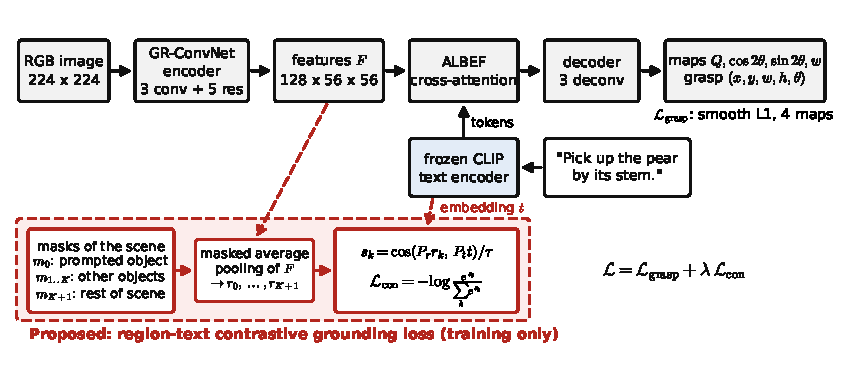
\includegraphics[width=0.66\linewidth]{fig/architecture.pdf}
  \caption{Top: the GR-ConvNet + CLIP baseline. Bottom (red, training only): the proposed loss.}
  \label{fig:arch}
\end{figure*}

\paragraph{Baseline.}
GR-ConvNet~\cite{kumra2020antipodal} encodes the $224 \times 224$ image into features $F \in \mathbb{R}^{128 \times 56 \times 56}$ and decodes four maps (quality $Q$, $\cos 2\theta$, $\sin 2\theta$, opening $w$); the grasp is read at the peak of $Q$.
Following~\cite{vuong2024language}, the prompt is encoded by a frozen CLIP text encoder~\cite{radford2021clip} and fused with the image by an ALBEF-style cross-attention layer~\cite{li2021albef}, where every position of $F$ attends to the text tokens (\cref{fig:arch}).
We place the fusion after the encoder (the paper does not say where), which gives 2.06M parameters, close to the 2.07M reported; $\mathcal{L}_{\mathrm{grasp}}$ is the sum of the smooth L1 losses of the four maps.

\paragraph{Region-text contrastive grounding.}
For a prompt about object $0$ of a scene, let $m_0$ be its mask, $m_1, \dots, m_K$ the masks of the other annotated objects, and $m_{K+1} = 1 - \max_k m_k$ the rest of the scene.
We pool the image-only features $F$ (before the fusion) over each region, project the regions and the pooled CLIP embedding $t$ of the prompt with two linear layers $P_r$ and $P_t$, and apply InfoNCE~\cite{oord2018cpc} with object $0$ as the positive:
\begin{equation}
  r_k = \frac{\sum_p m_k(p)\, F(p)}{\sum_p m_k(p)}, \qquad
  s_k = \frac{\cos(P_r r_k,\, P_t t)}{\tau},
  \label{eq:region}
\end{equation}
\begin{equation}
  \mathcal{L}_{\mathrm{con}} = -\log \frac{e^{s_0}}{\sum_{k=0}^{K+1} e^{s_k}}, \qquad
  \mathcal{L} = \mathcal{L}_{\mathrm{grasp}} + \lambda\, \mathcal{L}_{\mathrm{con}}.
  \label{eq:loss}
\end{equation}
The loss gives the encoder the semantic signal its grasp loss lacks.
The masks of all parts of an object are merged, since the part labels mostly repeat the object label (\cref{sec:experiments}).
$P_r$, $P_t$ and the masks are used in training only, so the inference network is unchanged.

\section{Experiments}
\label{sec:experiments}

\paragraph{Setup.}
The official split of the LGD code has 10,130 training, 515 Seen and 212 Unseen test objects with released labels (28.6k, 1,376 and 601 prompts; one prompt per sample).
We follow the authors' scripts: Adam, learning rate $10^{-3}$, batch 8, 50 epochs of 1,000 batches, model chosen on the Seen test; success means IoU $>$ 25\% and angle error $<30^{\circ}$ (opening scaled by 150); H is the harmonic mean.
$\lambda = 0.01$ (chosen among 0.01, 0.03, 0.1 on the Seen test), $\tau = 0.07$; mean $\pm$ std over seeds 123 to 125.

\paragraph{Notes on the official code.}
(i) The released evaluation feeds the object name, not the instruction our models read.
(ii) Its training and Seen evaluation both read \texttt{test/seen.obj}, so models re-run with it are compared on Unseen only.
(iii) Its GR-ConvNet + CLIP detaches the image features, so its encoder is not trained.

\begin{table}[t]
  \centering
  \small
  \setlength{\tabcolsep}{2.5pt}
  \begin{tabular}{@{}llccc@{}}
    \toprule
    Method & Text & Seen & Unseen & H \\
    \midrule
    LGD$^\dagger$~\cite{vuong2024language} & & 0.48 & 0.42 & 0.45 \\
    MaskGrasp$^\dagger$~\cite{vo2024maskgrasp} & & 0.50 & 0.46 & 0.48 \\
    GraspMamba$^\dagger$~\cite{nguyen2024graspmamba} & & 0.63 & 0.41 & 0.52 \\
    GraspSAM$^\dagger$~\cite{noh2024graspsam} & & 0.64 & 0.62 & 0.63 \\
    GR-ConvNet + CLIP$^\dagger$~\cite{vuong2024language} & & 0.37 & 0.18 & 0.24 \\
    \midrule
    LGD, released model$^\ddagger$ & name & - & \pend{x.xx} & - \\
    GR-ConvNet + CLIP$^\ddagger$ & name & 0.33$^\ast$ & 0.18 & - \\
    \midrule
    GR-ConvNet + CLIP & instr. & .331$\pm$.019 & .392$\pm$.017 & .358 \\
    + region-text contrastive & instr. & \textbf{.365}$\pm$.006 & \textbf{.403}$\pm$.032 & \textbf{.383} \\
    \bottomrule
  \end{tabular}
  \caption{Success rates. $^\dagger$Reported, other subsets (MaskGrasp H computed, GraspSAM Base / New). $^\ddagger$Re-run with the authors' code; $^\ast$Seen objects also in its training data. Last two rows: ours, 3 seeds. All but $^\dagger$: official split.}
  \label{tab:main}
\end{table}

\begin{table}[t]
  \centering
  \small
  \setlength{\tabcolsep}{4pt}
  \begin{tabular}{@{}lcccc@{}}
    \toprule
    & \multicolumn{2}{c}{Baseline} & \multicolumn{2}{c}{Ours} \\
    Gate & Seen & Unseen & Seen & Unseen \\
    \midrule
    None & 0.331 & 0.392 & 0.365 & 0.403 \\
    Grounding DINO box & 0.381 & 0.443 & 0.432 & 0.464 \\
    Ground-truth mask (oracle) & 0.468 & 0.518 & 0.543 & 0.565 \\
    \bottomrule
  \end{tabular}
  \caption{Grasp restricted to a region at inference, mean of 3 seeds.}
  \label{tab:gates}
\end{table}

\paragraph{Results.}
With $\lambda = 0.01$ the loss improves the baseline by 3.4 Seen, 1.1 Unseen and 2.5 H points, with an H gain in every seed (\cref{tab:main}); on all 13.5k labelled Unseen prompts of the Grasp-Anything list it is +0.9, again in every seed.
Larger weights are unstable: 0.375 $\pm$ 0.054 H for $\lambda = 0.03$, a collapse in one seed for $\lambda = 0.1$.
Re-run with the authors' code, the official GR-ConvNet + CLIP reaches 0.18 on Unseen (0.18 reported) and LGD \pend{x.xx} on a random subset of \pend{n} Unseen prompts (0.42 reported).
The oracle gate adds 12.6 Unseen points to the baseline and 16.2 to ours, and Grounding DINO 5.1 and 6.1 (\cref{tab:gates}): the two kinds of grounding combine.

\section{Conclusion}
\label{sec:conclusion}

Grounding is the main error of a reproduced baseline on Grasp-Anything++; our training-only contrastive loss improves unseen classes by 7.5 points, but mainly by reducing missed predictions, so grounding remains open.
Limitations: one seed per model, masks needed in training, no part-level grounding from the current labels, untuned $\lambda$ and $\tau$.

{
    \footnotesize
    \bibliographystyle{ieeenat_fullname}
    \bibliography{main}
}

\end{document}
